\chapter{ONLINE TRAINING FOR MOBILE OFFLOADING SCHEDULER}
\label{chap:online}
As I validated through detailed measurement experiments in Chapter V,
one important fact is that benefits and drawbacks from offloading
computation-intensive portions of mobile applications can be influences
by various internal and external factors, such as application
requirements, network conditions, and computing capabilities of mobile
and external devices.
%
Accordingly, \textit{whether to offload or execute locally} needs to be
decided dynamically based on internal and external conditions, and
monitoring the aforementioned dynamic features at runtime is required to
make offloading decisions.
%
Otherwise, incorrect offloading decisions may cause performance
degradation and/or increase energy consumption.
%
Related work has also considered dynamic scheduling for mobile
offloading frameworks.
%
For example, Kwon et al.~\cite{kwon} consider a simple threshold-based
scheduler in which the framework decides to offload  mobile
computations only when the data transfer size is higher than a certain
threshold.
%
MAUI~\cite{maui} utilizes a linear regression model using predefined
features, such as workload, network and device characteristics, to make
offloading decisions.\\
%
Even though these systems consider runtime schedulers for mobile
offloading, which take dynamic features such as data transfer size or
network conditions into account to make offloading decisions, it is
impractical for these approaches to build a generic offloading decision
policy embracing all possible cases over dynamic mobile environments.
%
For instance, consider that a mobile user walks around a shopping complex, while
receiving offloading-capable mobile services such as gaming or
augmented reality.
%
In this situation, network latency, bandwidth and availability can be changed from
moment to moment.
%
In addition, according to network conditions, the offloading service may
trigger the service migration to other remote servers, which may have
different computing power capabilities, to deliver better service experience
to the mobile user.
%
However, it is infeasible to define a static scheduling model by
expecting various network conditions and computing capabilities of remote
offloading servers.  
%
Furthermore, the scheduling policy, which is fitted with a particular
application, may not work correctly for other applications due to
different application requirements and characteristics.
%
For example, gaming and image processing applications may have different
computation complexity, though they process a similar size of data.\\
%
In this Chapter, I aim to develop a novel framework for an
adaptive runtime scheduler for mobile offloading by employing online
machine learning techniques -- MALMOS (machine learning-based mobile
offloading scheduler).
%
In this approach, a machine learning classifier makes decisions of
whether mobile computations should be offloaded to external resources,
or executed locally. 
%
To this end, I extend our work on offline machine
learning-based runtime scheduler~\cite{ml}, and develop a novel online
scheduling module in which any appropriate machine learning classifier
can be utilized for the runtime offloading scheduler.
%
Furthermore, MALMOS provides an online training mechanism for
the machine learning-based runtime scheduler such that it supports a
policy that dynamically adapts scheduling decisions at runtime based
upon the observation of previous offloading decisions and their
correctness.\\
%
To demonstrate its practical applicability, I integrated MALMOS
with an existing Java-based, offloading-capable code refactoring
framework, \textit{DPartner}~\cite{dpartner}.
%
Originally, the offloading-capable mobile applications generated by
DPartner depend on static (or user-provided) input to decide whether to
execute offloadable computations (i.e. Java classes) locally or remotely.
%
By combining the machine learning-based runtime scheduler with
these applications, offloading decisions are dynamic and do not require
any user input.
%
I have implemented an online-scheduled DPartner prototype, and used it
to perform quantitative experiments with Android mobile devices and
applications to evaluate the performance and cost for three machine
learning algorithms: instance-based learning, single layer perceptron, and na\"{i}ve
Bayes, with respect to classifier training time, classification time,
and scheduling accuracy.
%
Particularly, I examined the adaptability of MALMOS to various network
configurations and computing capabilities of remote resources by comparing
the scheduling accuracy with two static scheduling cases:
threshold-based and linear equation-based scheduling policies.
%
Even though there have been prior related studies which suggest
utilizing machine learning techniques for mobile computing environments,
to the best of our knowledge, our work is the first to consider an
online training mechanism for the machine learning-based runtime
scheduler, and to demonstrate with a end-to-end system performance and
cost of various machine learning algorithms for the runtime scheduler of
mobile offloading tasks.\\
%

\section{Background and Challenges}
\label{online:challenges}
%
In this section, I summarize our work on offline-trained
machine learning-based runtime scheduler for mobile offloading
framework.
%
Then, I describe challenges on the online training mechanism for the
machine learning-based runtime scheduler.
%

\subsection{Offloading Performance}
\label{online:performance}
In the previous Chapter, I studied a runtime scheduler for
mobile offloading framework through detailed measurement experiments.
%
With an OpenCL-based mobile offloading framework~\cite{ocloff}, I
performed various experiments using four different OpenCL workload
kernels used in a variety of areas such as image processing and
simulations.
%
Also, in order to observe the impact of different network conditions on
the offloading performance, I configured different network conditions:
local area network, campus network, and wide area network (i.e. Amazon
EC2 cloud).
%
In the evaluation, I verified that different network conditions result
in significant differences in offloading performance.
%
Also, each OpenCL workload kernel shows different offloading
performance, even though they process similar size of data, because each
kernel has different computational complexity.
%
These results demonstrated offloading performance
variation over different network conditions and OpenCL workload
kernels.\\
%
Based on our observation, I applied machine learning techniques
to runtime scheduling.
%
I trained various machine learning classifiers with
\textit{Weka}.
%
Then, I implemented a machine learning-based runtime scheduler by
building the trained machine learning classifiers onto the
OpenCL-based mobile offloading system.
%
In our evaluation, I observed that most of the machine learning-based
schedulers show scheduling accuracy higher than 80\%.
%

\subsection{Offline vs. Online Training}
\label{online:training}
There exist two possible ways to train the machine learning
classifier: \textit{offline} and \textit{online} training.
%
In offline training, the machine learning classifier can be trained
using a set of pre-collected static data.
%
Once the machine learning classifier is trained in the initial training
phase, the classifier does not change its prediction behavior.
%
It is therefore difficult to reflect unseen situations or conditions
which have not been trained in the initial training phase.
%
For that reason, offline machine learning should be trained through a
large set of data which covers as many cases as possible in order to
accomplish high prediction performance.\\
%
On the other hand, the online machine learning technique does
not depend on any pre-trained classifiers to predict the future
behaviors of the target system.
%
Instead, the online machine learning techniques trains its classifier
when a new data instance is available at runtime.
%
More specifically, the classifier of the online machine learning
technique is trained whenever the comparison result between the
prediction value and actual behavior is available.
%
Thus, the main challenge of online machine learning is to deliver the
prediction correctness into the training process, so that it can train
the classifier continuously based upon the prediction correctness feedback.
%
However, it can be too expensive to determine the correct prediction,
since the scheduler may have to attempt all of the possible decision
cases to know which prediction is correct.\\
%
In this Chapter, I extend our work on the offline
machine learning-based mobile offloading scheduler by considering an
adaptive online training mechanism.
%
In the case for the mobile offloading scheduler, even though
there exist only two possible cases (offloading and local processing),
the mobile platform still has to pay for both offloading and local
processing.  
%
Therefore, it is important to minimize the training cost while
guaranteeing reasonably acceptable scheduling performance.
%
This work addresses this challenge by proposing the adaptive online training
mechanism in which the training phase can be dynamically stretched and
shrunk according to the scheduling performance so that the mobile device
does not have to pay the unnecessary training cost by retaining a static
length of the training phase. 
%

\section{Architecture of MALMOS}
\label{online:architecture}
In this section, I describe the architecture and main modules of MALMOS.
%
Then, I describe implementation details on MALMOS with the adaptive
online training mechanism.
%
Lastly, I explain how MALMOS can be integrated with mobile offloading
frameworks, using DPartner as a concrete scenario.
%
The overall architecture and main modules of MALMOS are illustrated in
Figure~\ref{fig:malmos}.
%
The dotted lines indicate the application and network features flow path, and the
solid lines are the application computing tasks or scheduling-related
commands flow path.
%
\begin{figure}
\centering
\epsfig{file=figs/malmos.eps, width=4.0in}
\caption{Overall architecture of MALMOS with online training}
\label{fig:malmos}
\end{figure}
%

\subsection{Architecture and Modules of MALMOS}
\label{online:module}
As depicted in Figure~\ref{fig:malmos}, the overall architecture consists
of four main modules: computation dispatcher, runtime scheduler, machine
learning classifier, and the trainer for the machine learning classifier.
%
These four main modules interact with each other to schedule and
execute offloadable tasks, and to train the machine learning
classifier. 
%
At runtime, MALMOS operates alternatively in either of two different phases:
\textit{runtime scheduling phase} and \textit{online training phase}.
%
In the runtime scheduling phase, tasks are executed locally or remotely
based on the decisions from the scheduler.
%
First, the computation dispatcher receives an offloadable task
(\textcircled{1}).
%
%In the runtime scheduling phase, first, the computation dispatcher
%receives an offloadable computation (\textcircled{1}).
%
Then, according to the decision provided by the scheduler module
(\textcircled{2}), the dispatcher forwards this task to the appropriate
execution unit (\textcircled{3}): \textit{either} a local computing unit, or a
remote computing resource (through the network interface).\\
%
In contrast, in the online training phase, the machine
learning classifier is trained in accordance with the scheduling
performance (i.e. scheduling accuracy). 
%
In order to determine the scheduling performance, the offloadable
computation task is forwarded to and executed in \textit{both} execution
units; the computation dispatcher records both execution times, and
feeds back the performance comparison to the classifier trainer
({\textcircled{4}).
%
Based on this feedback from the dispatcher, the classifier trainer updates
the machine learning classifier ({\textcircled{5}).
%
The implementation details for these modules are as follows:\\
%
\textbf{Computation dispatcher.} This module has the
responsibility to dispatch and forward offloadable computation tasks to
the appropriate computing unit: remote computing resource (for offloading) or
local processing units (for local execution) according to the scheduling
decision from the scheduler module stored in the scheduling table.
%
In the online training phase, however, the computation dispatcher works
differently by forwarding and executing computation tasks in both local
processing units and remote computing resources.
%
Also, this module provides feedback to the classifier update in the
machine learning classifier trainer module, by comparing the performance
between offloading and local processing and feeding back which execution
leads to better performance.\\
%
\textbf{Machine learning classifier.} The machine learning classifier is
in charge of making decisions on offloading or local processing for
offloadable tasks.
%
The main difference, which distinguishes MALMOS from the previous
approaches on mobile offloading schedulers, is that it does not rely on
any predefined scheduling policies.
%
Instead, the machine learning classifier hooks up to the classifier
trainer, so the trainer updates the classifier at runtime whenever the feedback from
the computation dispatcher is available, and the machine learning
classifier adapts its decision behavior with changes of internal and
external environments.
%
When the scheduler module sends the request for offloading decisions
with the attributes obtained by the network and application profiler,
the machine learning classifier makes the decisions and stores them into
the scheduling table in the scheduler module.
%
Even though it is possible to adopt various attributes
from internal (application) and external (network, remote resources)
environments, for the current implementation, I employ two attributes:
the size of data to be sent to the remote resource, and the network
bandwidth.\\
%
\textbf{Runtime scheduler.} This module schedules the offloadable
computation tasks by sending the decision requests with the capture of
internal and external dynamic features.
%
Then, it stores the decision results from the classifier to the
scheduling table so that the computation dispatcher can forward each
computation tasks to the appropriate computing unit through looking up
the scheduling table.
%
Scheduling the computation tasks requires to profile internal
and external dynamic features, such as data size of inputs to the tasks
and network conditions. 
%
I achieved this profiling by implementing application and network
profilers.
%
For the application profiler, I defined an application programming
interface (API) to monitor the invocation of the offloadable computation
tasks and capture the size of input arguments.
%
Also, for the network profiler, I implemented network bandwidth
measurement by simply dividing the size of a probing packet with the elapsed
time to send the probing packet as described in~\cite{nws}.\\
%
However, profiling application and network conditions incurs
additional cost in terms of runtime overhead and energy consumption,
which means that too frequent profiling may lead to high overhead.
%
For this reason, I consider two scheduling strategies.
%
In the first strategy, each time offloadable tasks are invoked from the
mobile application, the runtime scheduler requests to make offloading
decisions while profiling application and network conditions.
%
I refer to this strategy as \textit{on-demand scheduling}.
%
Another strategy is \textit{periodic scheduling}, in which the
scheduler makes the decision requests asynchronously with actual
invocations of offloadable tasks, but periodically with a certain
interval.
%
Therefore, each profiler does not need to inspect application
and network conditions for every invocation of the offloadable tasks.
%
Also, in the periodic scheduling strategy, the scheduling interval
can increase and decrease dynamically according to network behavior
in order to obtain more up-to-date network conditions.
%
If the variation of network bandwidth is less than a threshold, which
can be thought as a steady-state network status, the scheduling interval 
becomes longer (e.g. twice as current interval).
%
The assumption is that it is likely that former scheduling can be 
still effective for the near future.
%
In contrast, if the variation of network bandwidth is greater than the
threshold, the interval becomes half of the current interval, leading to
more frequent scheduling.\\
%
\textbf{Machine learning classifier trainer.} With the feedback on the
performance comparison between offloading and local processing from the
computation dispatcher, the machine learning classifier trainer updates
the machine learning classifier.
%
In order to compare the performance between offloading and local
processing, the trainer creates one separate thread for local
processing, so that offloading and local processing can be executed
concurrently.
%
Then, the computation dispatcher measures the execution time for both
offloading and local processing to compare the performance and provides
the comparison result to the classifier updater. 
%
Finally, the classifier updater trains the machine learning classifier 
with the feedback from the computation dispatcher and the attributes
from the profilers.
%
\begin{figure}
\centering
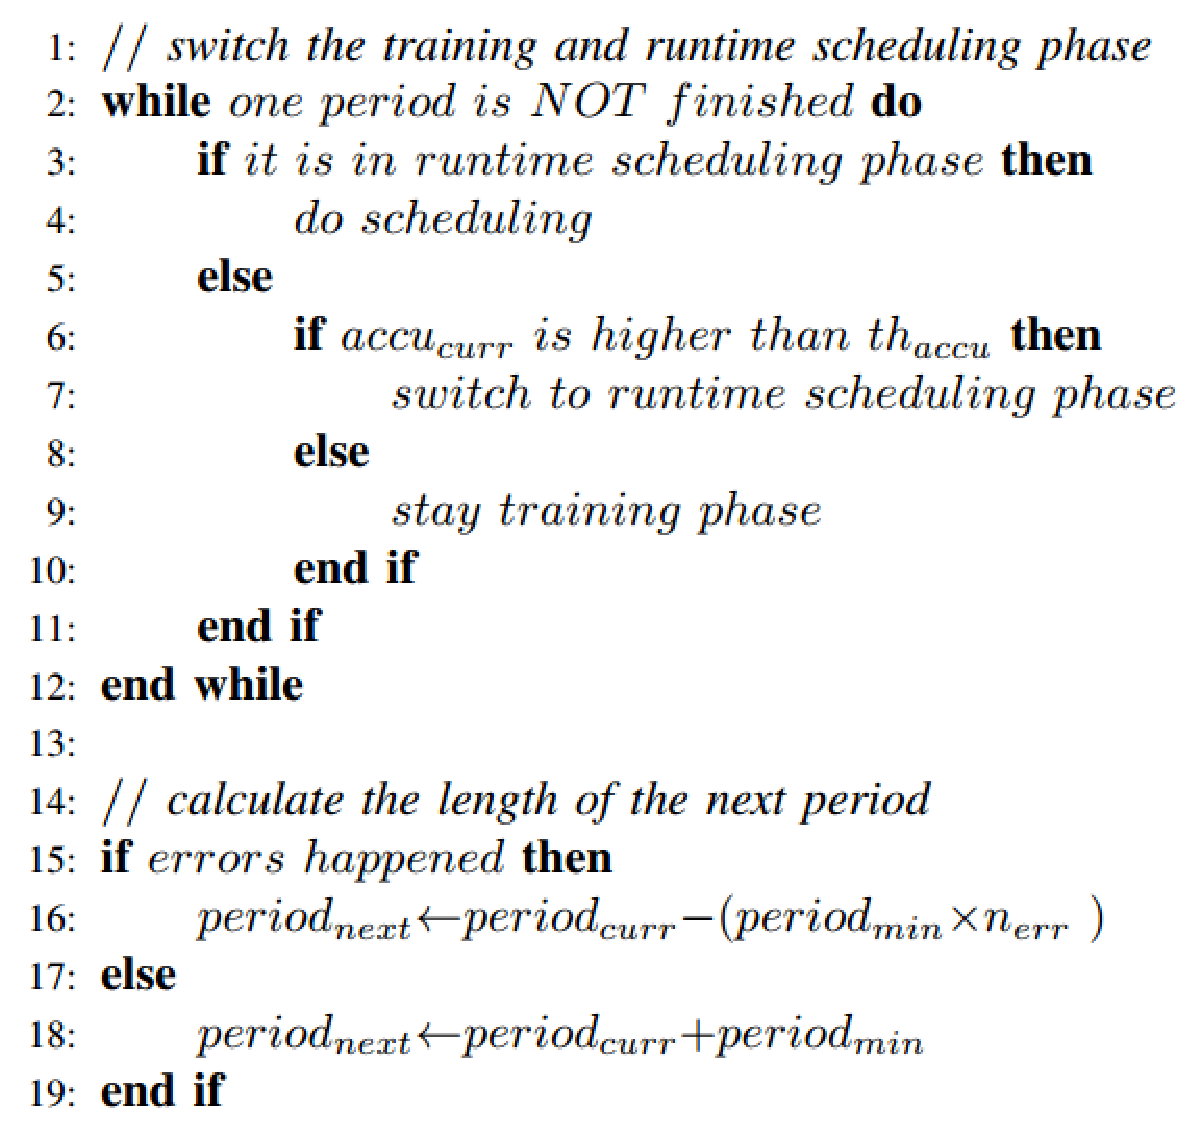
\epsfig{file=figs/malmos_algorithm.eps, width=4.0in}
\caption{Pseudo-code for adaptive online training mechanism}
\label{fig:malmos_algorithm}
\end{figure}
%

\subsection{Adaptive Online Training Mechanism}
\label{online:module}
One of the main contributions of this work is an adaptive online
training mechanism which allows the training phase duration to stretch
and shrink dynamically according to the scheduling accuracy.
%
The pseudo-code of the adaptive online training mechanism is shown in
Figure~\ref{fig:malmos_algorithm}.
%
First, lines 2--12 decide to switch the online training and runtime
scheduling phase by calculating the current scheduling accuracy.
%
In the training phase, if the current accuracy ($accu_{curr}$) is higher
than the accuracy threshold ($th_{accu}$), the online training mechanism
switches to the runtime scheduling phase.
%
Otherwise, it stays in the training phase.
%
Next, the length of the next period is calculated according to the
number of incorrect decisions (lines 15--19).\\
%
Figure~\ref{fig:malmos_example} illustrates an example of how the adaptive online
training mechanism works.
%
In this example, I set the accuracy threshold ($th_{accu}$) to 70\% and
the minimum length of one period to 5 to make the explanation clear to
understand at a glance.
%
Also, I assume that there is no incorrect decision or scheduling error
in the first, second, and fourth period, but one error in the third
period.
%
In order to measure the current scheduling accuracy ($accu_{curr}$) of
the classifier, the trainer observes whether the performance comparison
matches with the offloading decision.
%
For example, if the classifier makes a decision to offload and
offloading actually has better performance than local processing, I
regard this case as a correct decision.
%
Then, I calculate the current scheduling accuracy using
Equation~\eqref{equ:accuracy}.
%
\begin{figure}
\centering
\epsfig{file=figs/malmos_example.eps, width=4.5in}
\caption{An example of the adaptive online training mechanism}
\label{fig:malmos_example}
\end{figure}
%
\begin{equation}
	accu_{curr} = N_{correct}\:/\:(N_{total} + 1)
\label{equ:accuracy}
\end{equation}
%
where $N_{correct}$ and $N_{total}$ are the number of correct decisions
and total decisions.
%
I add one to the denominator in order to avoid 100\% of
scheduling accuracy at just one training (if the decision is correct in
the first training turn, the scheduling accuracy becomes 100\%).\\
%
In Figure~\ref{fig:malmos_example}, the runtime scheduling phase begins after three
training turns in the first and second period because the scheduling
accuracy at third training turn is 75\% which is higher than 
$th_{accu}$, 70\%.
%
Furthermore, because there was no decision error in the first and second
period, the next length of one period increases by adding the
minimum length of one period.
%
Thus, the lengths of the second and third period become 10 and 15,
respectively.
%
In the third period, however, as one incorrect decision has
occurred, the training phase holds for six executions when the
scheduling accuracy becomes higher than 70\%, and the length of the
fourth period decreases by the minimum length of one period multiplied
by the number of incorrect decisions (in this case, 1).
%
This adaptive online training mechanism is inspired by the concept of
the feedback control algorithm used for TCP congestion avoidance called
\textit{Additive Increase Multiplicative Decrease}.
%

\subsection{Integration with On-Demand Java-based Offloading Framework}
\label{online:integration}
To demonstrate the applicability of this approach, I integrated the
modules of MALMOS into the DPartner mobile application framework, which
is capable of automatically refactoring Java-based mobile applications
to identify offloadable computation tasks.
%
Given an Android mobile application, first of all, DPartner examines its
bytecode to classify the Java classes into the anchored and offloadable
classes, so it can be guaranteed that the anchored classes are executed
on the mobile device while directly using a variety of the local sensors
such as the GUI display, camera, accelerator, and GPS.
%
Also, DPartner rewrites the bytecode for the offloadable classes to
implement a special type of the program structure to support on-demand
offloading.
%
Then, DPartner packages the files such as images, xml files, external
libraries, and rewritten bytecode for the offloadable classes, and
generates two separate objects which are deployed into the mobile device
and the remote server, respectively.\\
%
With respect to scheduling, the offloading-capable
Android applications generated by DPartner require either static or
user-provided decisions. 
%
However, static scheduling becomes inaccurate if conditions change, and
it is impractical that the mobile user monitors internal and
external environments and schedules each offloadable mobile computations
at runtime.
%
I address this challenge by integrating MALMOS with the
offloading-capable mobile applications generated by DPartner. 
%
I was able to achieve this integration without requiring deep
modifications or code additions to DPartner.
%
In fact, the only major code addition is to define new APIs to acquire
the data size of offloadable computations and the network bandwidth. 
%
By combining MALMOS with these applications, the mobile user can be free
of the burden of scheduling tasks.
%

\section{Evaluation}
\label{online:evaluation}
In this section, I evaluate the prototype implementation of MALMOS with
respect to the scheduling performance and cost.
%
First, I examine the training and classification time for different
categories of machine learning algorithms: instance-based learning,
single layer perceptron, and na\"{i}ve Bayes.
%
I examined the adaptability of MALMOS to various network conditions and
computing capability of remote resources by comparing the scheduling
accuracy with two static scheduling cases: threshold-based and linear
equation-based scheduling policies, by running three synthetic
applications (hidden Markov model, floating-point matrix multiplication, and
sobelfilter) and two real applications (Linpack and Go game).
%
\subsection{Experimental setup}
\label{online:setup}
Even though high-dimensional machine learning algorithms (such as
decision tree, multi layer perceptron, or support vector machine) can
achieve more accurate scheduling performance, they might be too
expensive to be used for mobile platforms.
%
Based on algorithm complexity considerations, I selected three machine learning
algorithms: instance-based learning, single layer perceptron, and
na\"{i}ve Bayes for out prototype implementation.\\
%
Also, in order to evaluate the adaptability of MALMOS to various
network conditions and computing capabilities of remote computing
resources, I setup experiments using a variety of hardware and
network configurations.
%
First of all, our hardware setup consists of a mobile client and three
different remote servers.
%
I have utilized an Android smartphone, Nexus 5 equipped with 2.3Ghz
quad-core processor and 2GB RAM, and running Android KitKat as the
mobile client.
%
For the remote servers, I used two laptops and one desktop which have
different levels of computing power capabilities.
%
The first laptop has an Intel i5 Quad core 2.6Ghz processor and 8GB RAM, while
the second laptop is equipped with an Intel Core2 Duo 2.0Ghz processor and 2GB
of memory.
%
In addition, I ran CPU-intensive workloads on the second laptop using
\textit{Stress}, a simple workload generator~\cite{stress}, to observe 
the effect of CPU load at the remote resource on the scheduling performance.
%
The third remote resource is a workstation with an Intel Core2 Duo 3.0Ghz processor
and 8GB RAM.
%
All remote servers run Linux OS, Ubuntu 12.04.\\
%
Instead of installing the aforementioned three remote servers in
different network environments, for the network configurations, I
emulated three different network bandwidth characteristics: local area
network, campus network, and wide area network by using the Traffic
Control (TC) tool as described in Table~\ref{table:network_summary}.
%
The experimental setup using TC gives flexibility to vary network
conditions between the mobile device and remote resources.\\
%
I experiment three synthetic applications: hidden Markov
model, floating-point matrix multiplication and sobelfilter, and two real
applications available in Google Play: Linpack~\cite{linpack} and 
Go game~\cite{go}, each having different application requirements 
and computation complexities.
%
For example, sobelfilter is an image edge detection filter; it
takes a relatively large size of input, while its computation complexity
is low.
%
Therefore, I classify sobelfilter as a communication-intensive
application.
%
In contrast, the core computation of Go game is a Monte Carlo
algorithm with iterative random sampling tasks which have high
computation complexity.
%
Thus, Go game is a computation-intensive application.
%
Otherwise, the computation complexity of other three applications
depends on the size of input such as matrix size (for floating-point matrix
multiplication and Linpack), and the number of states (for hidden Markov
model).
%
\begin{figure}
\centering
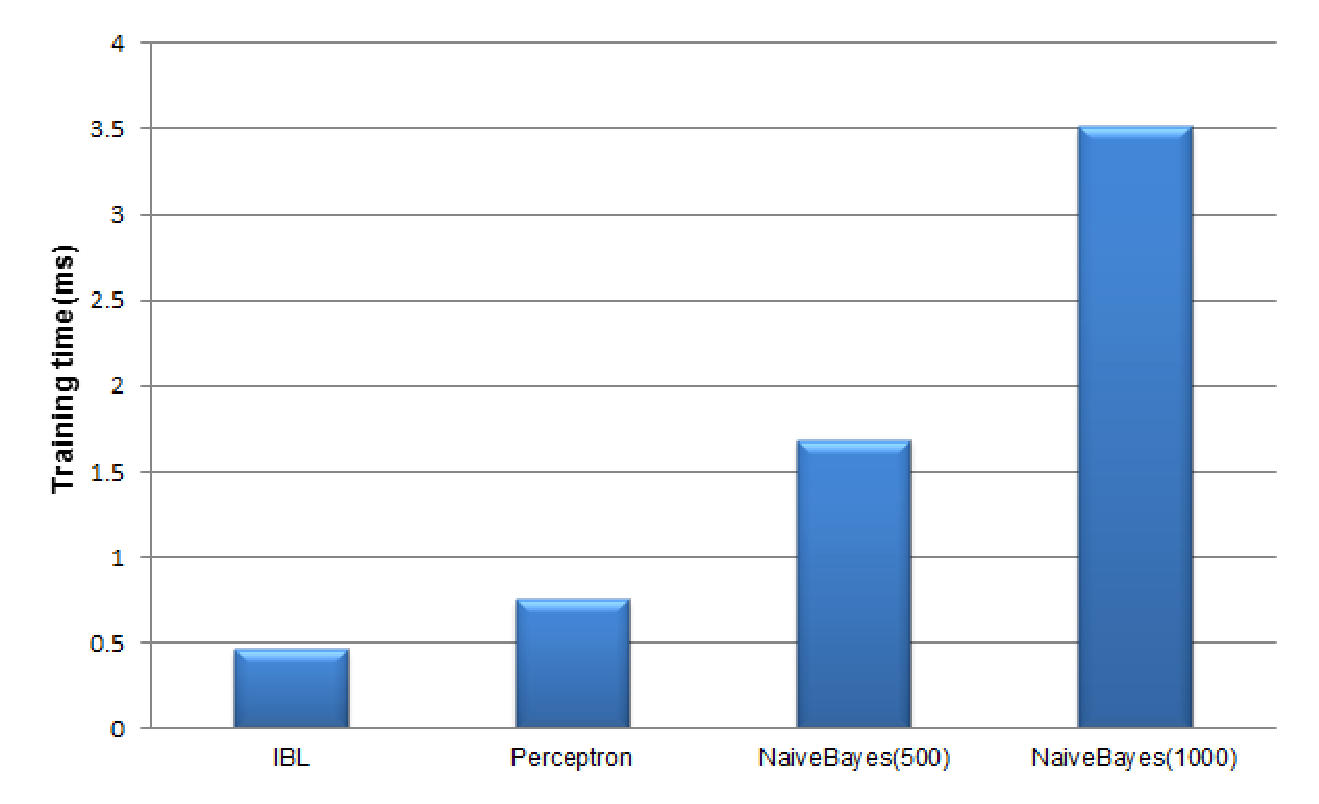
\epsfig{file=figs/training.eps, width=4.5in}
\caption{Training time comparison for three machine learning algorithms}
\label{fig:training}
\end{figure}
%
\begin{figure}
\centering
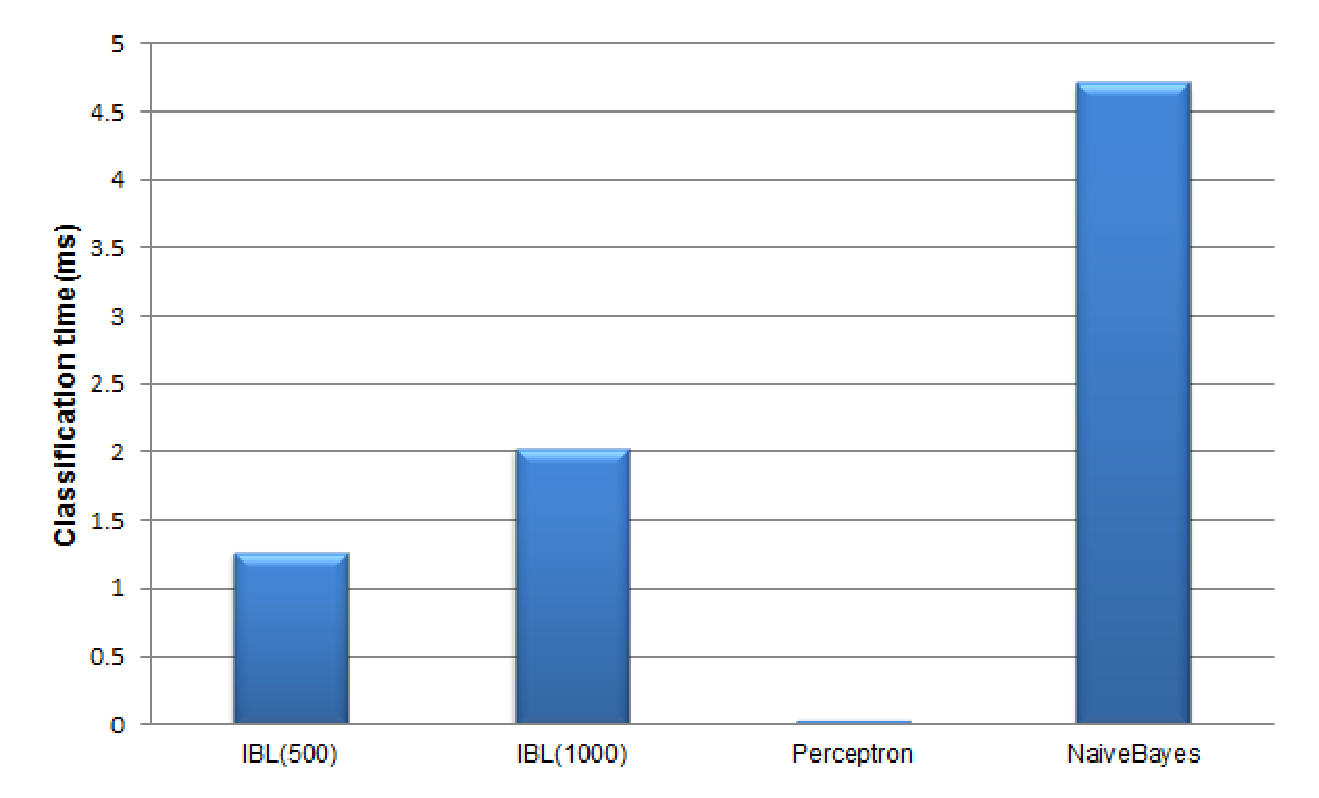
\epsfig{file=figs/classification.eps, width=4.5in}
\caption{Classification time comparison for three machine learning algorithms}
\label{fig:classification}
\end{figure}
%

\subsection{Overhead of training anc classification}
\label{online:overhead}
Since our machine learning-based mobile offloading scheduler keeps
training the classifier, which leads to runtime overhead, I
measured the cost to train the machine learning classifier.
%
As shown in Figure~\ref{fig:training}, instance-based learning has the shortest
classifier training time among three machine learning algorithms.  
%
In fact, the basis for the classification of instance-based learning is
the instance database, where previously experienced cases are stored.
%
Instead of training the explicit classifier, therefore, instance-based
learning adds a new instance to the database for the future
classification, resulting in relatively small training overhead.
%
On the other hand, na\"{i}ve Bayes with 1000 instances of database has
the largest training overhead. 
%
From the algorithm perspective, na\"{i}ve Bayes measures the
probability density for the given classes with the mean and standard
deviation, and chooses the class with the highest probability.
%
Thus, na\"{i}ve Bayes calculates the mean and standard deviation
throughout the previous instances for each class whenever a new instance
is trained.
%
Consequently, na\"{i}ve Bayes with 1000 instances, which requires
relatively heavy calculations for the mean and standard deviation, has
bigger training overhead than other machine learning algorithms.\\
%
Also, Figure~\ref{fig:classification} shows the classification time that the machine
learning classifier consumes to make a decision.
%
Similarly as the training time, na\"{i}ve Bayes shows bigger overhead
than other machine learning algorithms.
%
I used the Gaussian distribution to calculate the probability
density for each class with the mean and standard deviation value.
%
Therefore, the classification for na\"{i}ve Bayes entails complex
arithmetic operations, such as the exponential function and the square
root, which take longer than addition, multiplication, or comparison.
%
For that reason, na\"{i}ve Bayes has the largest classification overhead.
%
Note that perceptron has remarkably low classification overhead compared
with other machine learning algorithms. 
%
For perceptron, the classification process involves calculating the
output from a multivariable linear equation consisting of the attributes
weighted by the coefficients, which requires small amount of
the computation. 
%
As a result, perceptron shows the lowest cost in terms of the
classification time amongst three machine learning algorithms by showing
less than 0.05ms of the classification time.
%

\subsection{Scheduling Accuracy}
\label{online:accuracy}
I then investigated the scheduling accuracy of the three machine learning
algorithms.
%
For an unbiased evaluation, I turned off the adaptive online training
mechanism, and the online training phase and runtime scheduling phase were
uniformly switched in one period (5 of training and 15 of runtime
scheduling).
%
A total of 10 periods were repeated for the average.
%
Also, I demonstrated the adaptability of MALMOS to various network
conditions and computation capability of remote resources by comparing
with two static scheduling policies: threshold-based and linear
equation-based scheduling cases.
%
For the threshold-based scheduler, I empirically observed the
performance for offloading and local processing and picked up the input
size where the execution time of offloading or local processing comes from
behind the other.
%
For instance, if the matrix size is bigger than 170$\times$170,
offloading matrix multiplication to the workstation located in local
area network shows better performance than local processing.
%
As a result, I selected the data size corresponded with 170$\times$170 of matrix
size (i.e. 231KBytes) as the threshold so that when the data size is bigger than the
threshold, the scheduler makes decision to offload the computation.   
%
Therefore, the threshold-based scheduler does not account for the network
conditions.
%
For the case of the linear equation-based scheduling policy, I
established a two dimensional linear equation that distinguishes the
cases where offloading or local processing has better performance than
the other.
%
In order to define this linear equation, I gathered the performance of
offloading each application to the workstation varying the network
bandwidth.
%
In this experimental setup, I measured the scheduling accuracy by
offloading each application to four different remote servers, while
varying the network bandwidth and the size of input.
%
In order to change the network bandwidth, I wrote a simple script file
in which the TC command randomly switches among the three network
bandwidth described in Table~\ref{table:network_summary} in a certain interval during the
experiment.\\
%
\begin{figure}
\centering
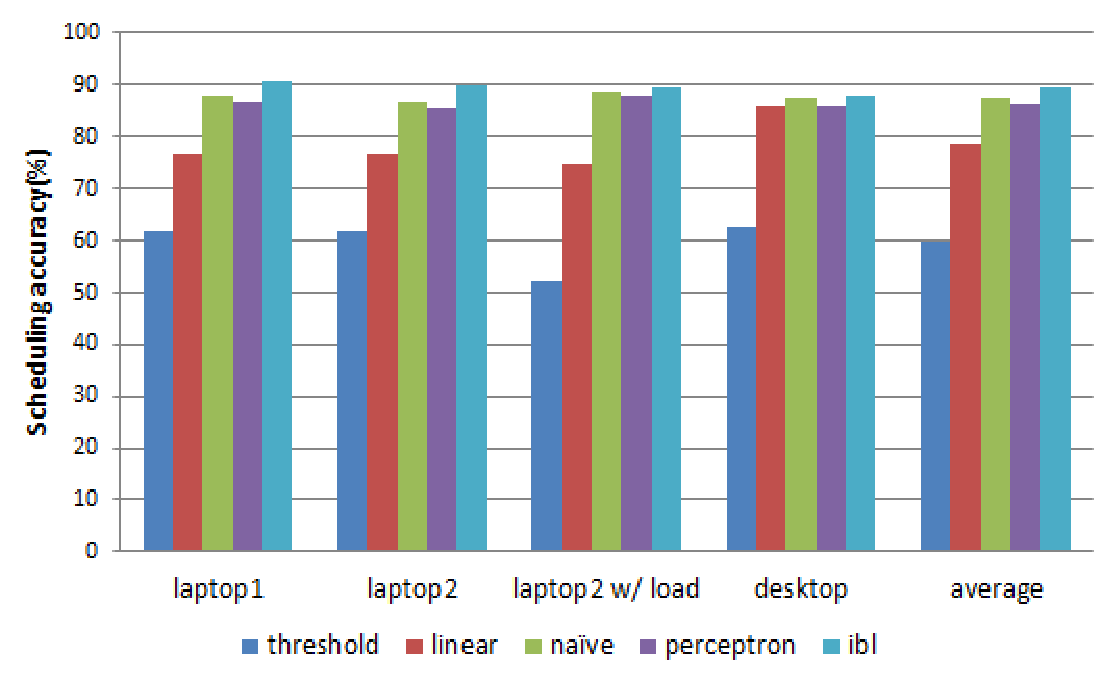
\epsfig{file=figs/scheduling_hmm.eps, width=5.0in}
\caption{Scheduling accuracy for hidden Markov model with various
configurations}
\label{fig:scheduling_hmm}
\end{figure}
%
\begin{figure}
\centering
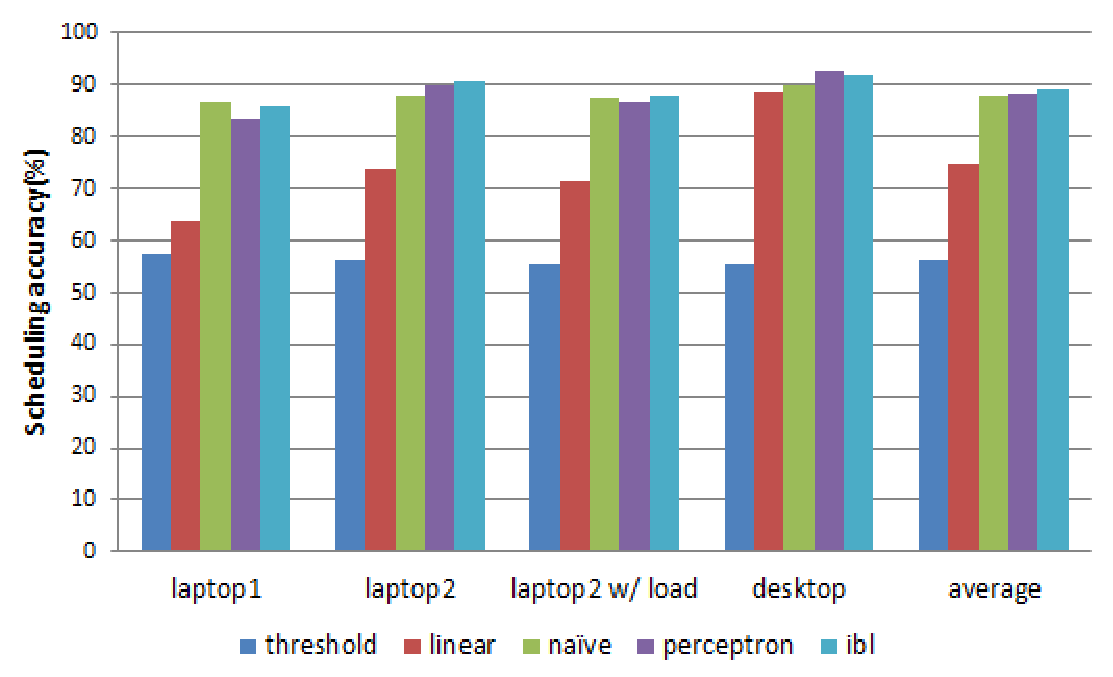
\epsfig{file=figs/scheduling_matrix.eps, width=5.0in}
\caption{Scheduling accuracy for matrix multiplication with various
configurations}
\label{fig:scheduling_matrix}
\end{figure}
%
\begin{figure}
\centering
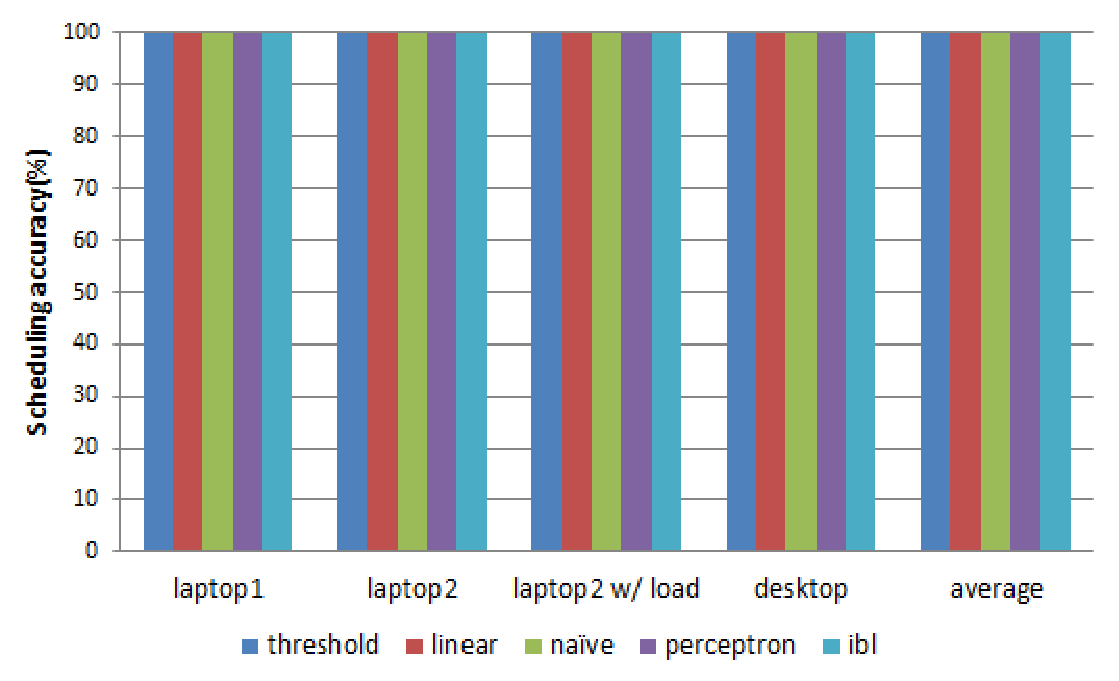
\epsfig{file=figs/scheduling_sobel.eps, width=5.0in}
\caption{Scheduling accuracy for sobelfilter with various
configurations}
\label{fig:scheduling_sobel}
\end{figure}
%
\begin{figure}
\centering
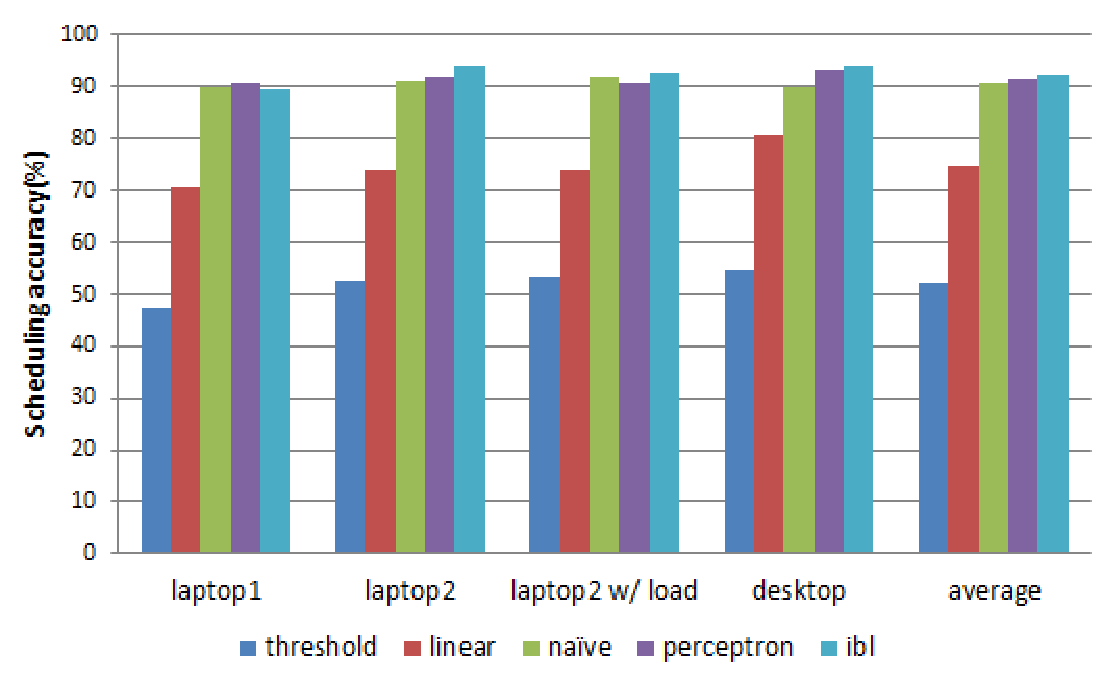
\epsfig{file=figs/scheduling_linpack.eps, width=5.0in}
\caption{Scheduling accuracy for Linpack with various
configurations}
\label{fig:scheduling_linpack}
\end{figure}
%
\begin{figure}
\centering
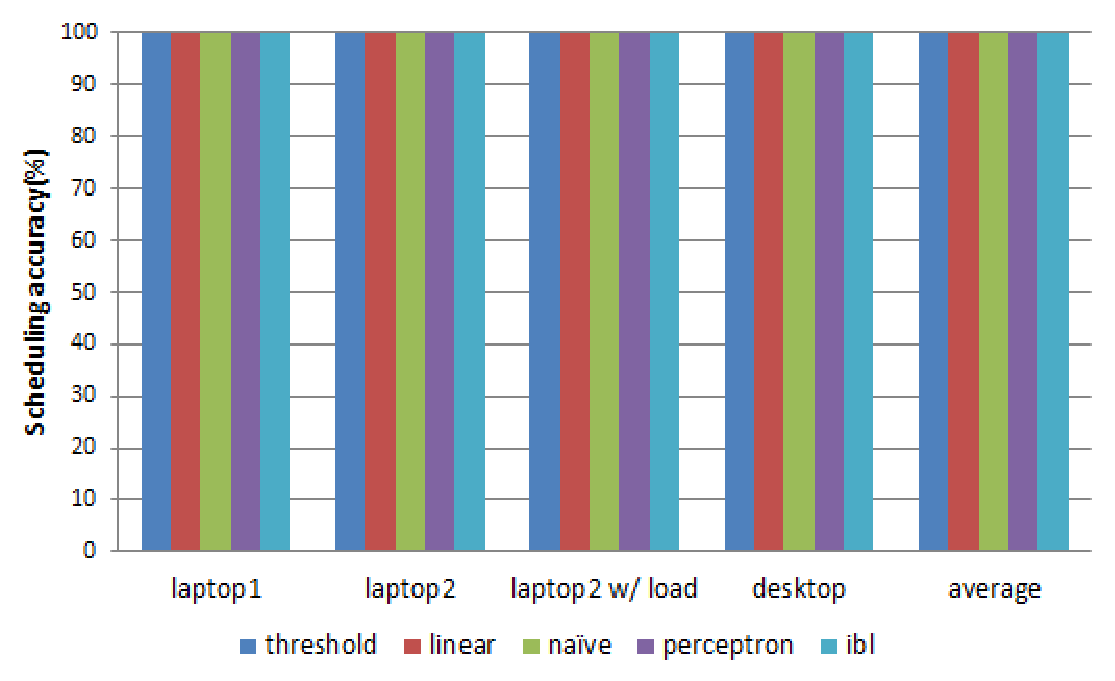
\epsfig{file=figs/scheduling_gogame.eps, width=5.0in}
\caption{Scheduling accuracy for Go game with various
configurations}
\label{fig:scheduling_gogame}
\end{figure}
%
As shown in
Figure~\ref{fig:scheduling_hmm},~\ref{fig:scheduling_matrix},
and~\ref{fig:scheduling_linpack}, MALMOS with
instance-based learning, perceptron, and na\"{i}ve Bayes has better
scheduling performance than the threshold-based and linear
equation-based scheduling policies in the cases of hidden Markov model,
matrix multiplication, and Linpack by showing averagely 86\%$\sim$92.5\% of the
scheduling accuracy over four remote resources setups.
%
The threshold-based scheduler considers only the
size of input data as the decision factor, but does not reflect the
dynamic network bandwidth.
%
Consequently, the threshold-based scheduler shows the poorest scheduling
performance in all experimental scenarios.
%
Particularly, the linear equation-based scheduling policy has similar
performance as three machine learning-based schedulers in the cases of
offloading applications to the workstation, since the linear
equation-based scheduler has been defined based on the offloading
performance with the workstation while varying the network bandwidth.
%
Nevertheless, the linear equation-based scheduler shows poor
scheduling accuracy (ranging from 64\%$\sim$76.6\%) in other remote server
setups, such as laptop or laptop with CPU load.
%
This is because other remote servers have different computing power
capabilities, hence the offloading performance can be quite different
with the case of offloading to the workstation.\\
%
On the other hand, Figure~\ref{fig:scheduling_sobel}
and~\ref{fig:scheduling_gogame} show that all scheduling
cases have exactly 100\% of the scheduling accuracy for sobelfilter and Go game.
%
As I mentioned earlier, sobelfilter and Go game are the
communication-intensive and computation-intensive application,
respectively.
%
For this reason, sobelfilter always prefers local processing and Go game
always prefers offloading.
%
Even in these extremely simple cases, MALMOS demonstrates the scheduling
performance as good as the threshold- and linear equation-based
scheduler.
%
It is worth noting that I established different threshold values and linear
equations for each application. 
%
Even though I used three machine learning algorithms for each
application without any change, MALMOS works universally well in all of
our experimental setup.\\
%
To evaluate end-to-end application performance, I measure the
offloading time of Linpack.
%
\begin{figure}
\centering
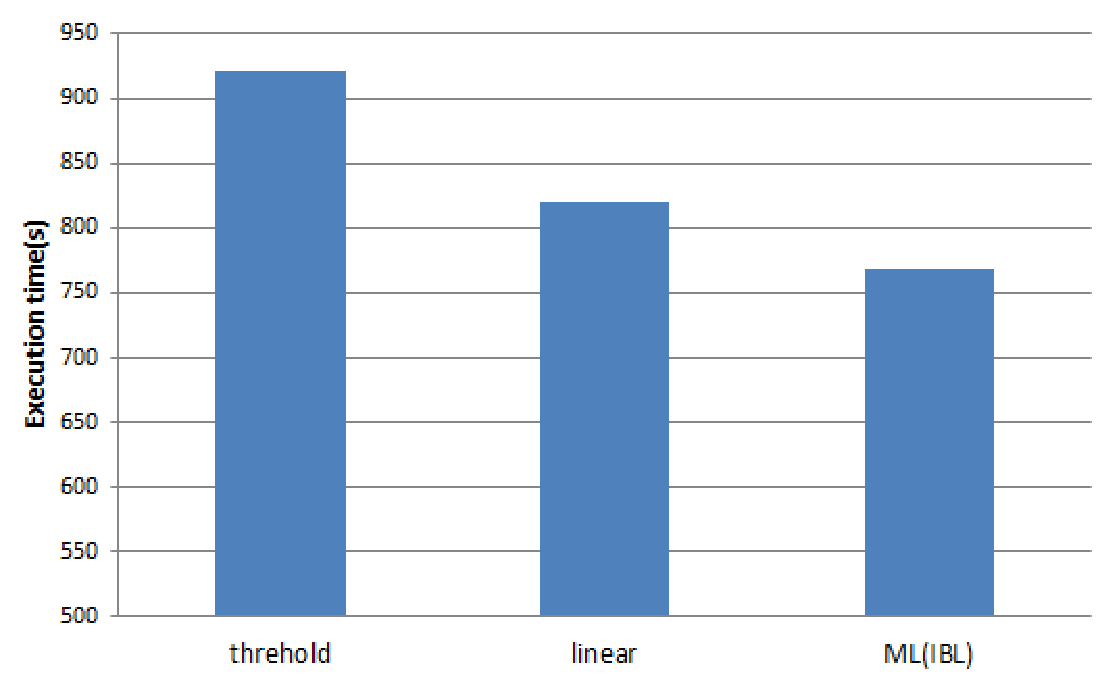
\epsfig{file=figs/execution.eps, width=4.5in}
\caption{Total execution time of 150 Linpack runs}
\label{fig:execution}
\end{figure}
%
Figure~\ref{fig:execution} shows total execution time of 150 Linpack runs with
the threshold-based, linear equation-based, and MALMOS (instance-based
learning).
%
For this experiment, I used the threshold- and linear equation-based
scheduling policies derived from the observation of the offloading
performance with the workstation as the remote resource.
%
With three scheduling policies, the mobile devices offloads Linpack to
the laptop equipped Intel Core2 Duo 2.0Ghz processor running CPU load by
Stress, while changing the network bandwidth as described in the previous 
experiment, and I measured tatal execution time of 150 Linpack runs with 
different input date size. 
%
As shown, the threshold-based scheduler has the longest execution
time due to the lowest scheduling accuracy.
%
The linear equation-based scheduler also shows 6.5\% longer execution
time than MALMOS. 
%

\section{Summary}
\label{online:summary}
%
In this Chapter, I proposed a novel machine learning-based mobile offloading
scheduler with online training, MALMOS.
%
MALMOS is designed in a modular fashion to generally apply to any types of mobile
offloading frameworks.
%
Also, I proposed an adaptive online training mechanism in which the
online training phase and runtime scheduling phase are dynamically switched
according to the scheduling accuracy.
%
To evaluate our work, I applied MALMOS to DPartner, a Java-based on-demand
offloading framework.
%
Also, I utilized three different machine learning algorithms for the
scheduling classifier and compared the overhead in terms of the training
and classification time.
%
Furthermore, I validated the ability of MALMOS to adapt to various network
conditions and computing power capabilities of the remote computing resources
by comparing the scheduling performance with threshold- and linear
equation-based scheduling policies.
%
In the evaluation, I observed that MALMOS has 10.9\%$\sim$40.5\% higher
scheduling performance than two static scheduling policies under various
network conditions, computing power capabilities of the remote servers, and
application complexity.\\
%











